\documentclass[11pt,a4paper]{article}
\usepackage[T1]{fontenc}
\usepackage[utf8]{inputenc}
\usepackage{lmodern,microtype}
\usepackage[margin=27mm,headheight=14pt]{geometry}
\usepackage{amsmath,amssymb,amsthm,mathtools}
\usepackage{booktabs,longtable,array,enumitem,graphicx}
\usepackage{xcolor,xurl,hyperref,fancyhdr,etoolbox}
\makeatletter
\patchcmd{\l@section}{1.5em}{2.2em}{}{}
\renewcommand*\l@subsection{\@dottedtocline{2}{2.2em}{2.7em}}
\makeatother
\definecolor{inkblue}{HTML}{183B56}
\definecolor{linkblue}{HTML}{135F91}
\hypersetup{colorlinks=true,linkcolor=inkblue,citecolor=linkblue,
 urlcolor=linkblue,pdftitle={Resonant Order Jets and Inverse Transseries for Polylogarithms},
 pdfauthor={Research draft prepared for Vladimir Reshetnikov}}
\pagestyle{fancy}
\fancyhf{}
\fancyhead[L]{\small Polylogarithms and inverse transseries}
\fancyhead[R]{\small\thepage}
\setlength{\emergencystretch}{2em}
\setlength{\parskip}{3pt}
\setlist{itemsep=3pt,topsep=5pt}
\numberwithin{equation}{section}
\newtheorem{theorem}{Theorem}[section]
\newtheorem{proposition}[theorem]{Proposition}
\newtheorem{lemma}[theorem]{Lemma}
\newtheorem{corollary}[theorem]{Corollary}
\theoremstyle{definition}
\newtheorem{definition}[theorem]{Definition}
\newtheorem{example}[theorem]{Example}
\theoremstyle{remark}
\newtheorem{remark}[theorem]{Remark}
\DeclareMathOperator{\Li}{Li}
\DeclareMathOperator{\Log}{Log}
\DeclareMathOperator{\Rea}{Re}
\DeclareMathOperator{\Ima}{Im}
\DeclareMathOperator{\Res}{Res}
\newcommand{\C}{\mathbb C}
\newcommand{\N}{\mathbb N}
\newcommand{\Nzero}{\mathbb N_0}
\newcommand{\dd}{\,d}
\newcommand{\eps}{\varepsilon}
\newcommand{\zder}[2]{\zeta^{(#1)}(#2)}
\newcommand{\coef}[2]{[#1]\,#2}
\newcommand{\LiInv}{\ell}
\newcommand{\repoCommit}{9ec0f0406afe7a5475b03ff65ed91f7e283979b8}

\title{\color{inkblue}\bfseries Resonant Order Jets and\\
Convergent Inverse Transseries\\[4pt]
\large for Polylogarithms and Logarithmically Weighted Tails}
\author{Research draft prepared for Vladimir Reshetnikov\\
\small A contribution for the ProveIt research collection}
\date{12 October 2026}

\begin{document}
\maketitle
\begin{abstract}
We study the inverse of a polylogarithmic endpoint deficit and the changes
in its transseries when the order passes through an integer.  An exact
pole-cancellation formula expresses every resonant order derivative in
terms of complete Bell polynomials, harmonic numbers, zeta values and
Stieltjes constants.  For higher integer orders, the inverse is a
convergent logarithmic series with a sharp degree bound.  Its highest
logarithmic coefficients obey a universal Fuss--Catalan law, including
arbitrary fixed nonnegative integer logarithmic weights.

At the critical order two, we construct a single holomorphic inverse
chart for the weighted deficit
\(\sum_{\nu\ge1}(\log\nu)^k(1-e^{-\nu t})/\nu^{2+\eps}\).
It is uniform when \(\eps\log(1/y)\) stays in a compact real interval and
converges in three independent small variables.  The construction gives
all inverse-logarithmic and exponential blocks, an explicit first
correction, and the first possible exponentially smaller block.

We also give a self-contained global contour argument for coefficients
of the ordinary compositional inverse.  It identifies two missing
normalization factors in the author-hosted 10 February 2025 note of
Krattenthaler and Rivoal.  For orders at least three, the entire
coefficient expansion has a sharp logarithmic support boundary with
explicit Fuss--Catalan coefficients.  For the dilogarithm, an all-orders
expansion in an exact Lambert variable has coefficients given by
derivatives of the reciprocal Gamma function at negative integers.
Convergent local charts are carefully distinguished from these outer
asymptotic expansions.  The accompanying code provides exact algebraic
checks and independent high-precision numerical diagnostics.
\end{abstract}

\noindent\textbf{Status.}
The results are proved below in conventional mathematical prose.
The proposed contributions are measured against the explicitly inspected
repository material and primary sources; worldwide priority is not
claimed.  No Lean formalization is claimed.  The numerical diagnostics
are not interval certificates.

\clearpage
\begingroup
\small
\setlength{\parskip}{0pt}
\tableofcontents
\endgroup
\newpage

\section{Research question, contributions, and provenance}
\label{sec:intro}

The natural common ground between polylogarithms and transseries is not
only the large-argument expansion of a special function.  It is also the
local inverse problem at a singular endpoint.  The classical formula
\[
 \Li_s(e^{-t})
 =\Gamma(1-s)t^{s-1}
   +\sum_{j\ge0}\zeta(s-j)\frac{(-t)^j}{j!}
\]
contains a fractional power for nonintegral \(s\).  At a positive integer,
the Gamma pole and one zeta pole cancel and leave a logarithm.
Inversion turns this elementary collision into a structured family of
power--logarithm series.  Differentiation in \(s\) raises the logarithmic
degree, while the limit \(s\to2\) changes the leading inverse scale.

Three distinctions guide the paper.  First, an exact identity of
holomorphic germs is stronger than a formal reversion.  Second, a
convergent expansion in several independent small variables may become
a transseries after those variables are related.  Third, coefficient
extraction from such a germ generally produces a new asymptotic
expansion; convergence of the original chart does not establish
convergence of that outer expansion.

\subsection{Main results}

For orientation, the principal conclusions are the following.

\begin{enumerate}
\item \textbf{All resonant order jets.}
Theorem~\ref{thm:jets} gives an exact, normally convergent formula at every
positive integer order.  Its logarithmic polynomial is an explicit
complete Bell polynomial.  This is a systematic derivation from the
classical Jonqui\`ere expansion, with all signs and removable limits fixed.

\item \textbf{Weighted logarithmic inverse and its sharp boundary.}
For \(m\ge2\), \(k\ge0\), and
\[
 D_{m,k}(t)=\sum_{\nu\ge1}
 \frac{(\log\nu)^k(1-e^{-\nu t})}{\nu^{m+1}},
\]
Theorem~\ref{thm:weighted-inverse} proves a convergent expansion
\(t(y)=\sum_{N\ge1}y^NT_N(\log y)\), with
\[
 \deg T_N\le(k+1)\left\lfloor\frac{N-1}{m-1}\right\rfloor.
\]
The bound is attained on an infinite set of indices.  The corresponding
coefficients are given exactly by Fuss--Catalan numbers.

\item \textbf{Uniform weighted transition through order two.}
Theorem~\ref{thm:critical} gives a convergent analytic chart for
\(D_{\eps,k}(t)=y\), uniformly in
\(\tau=\eps\log(1/y)\) on compact real intervals.  The leading scale is
\[
 t\sim \frac{y}{T^{k+1}H_k(\tau)},\qquad
 T=\log(1/y),\qquad H_k(\tau)=\int_0^1u^ke^{-\tau u}\dd u.
\]
All three small variables and their exact implicit equation are given.
The first correction and the first exponential block are explicit.

\item \textbf{Corrected and refined inverse coefficient asymptotics.}
If \(\Li_s(\LiInv_s(w))=w\) near zero and
\(a_n^{(s)}=[w^n]\LiInv_s(w)\), then
\[
 a_n^{(2)}\sim-\frac{\zeta(2)^{1-n}}{n^2(\log n)^2},
 \qquad
 a_n^{(s)}\sim
 -\frac{\zeta(s)^{s-1-n}}{\zeta(s-1)^s n^s}
 \quad(s\in\{3,4,\ldots\}).
\]
Theorem~\ref{thm:coeff-higher} gives an all-orders refinement and its
highest-logarithm coefficients.  Theorem~\ref{thm:coeff-dilog} gives
the dilogarithmic expansion in a Lambert variable, with a reciprocal
Gamma coefficient formula.
\end{enumerate}

\subsection{Relation to the inspected ProveIt material}

The repository was read at commit
\[
 \texttt{\repoCommit}.
\]
The scope of the inspection is recorded in the accompanying provenance
file.  It includes the Polylogarithms manuscript chapters and the
relevant Transseries reports, rather than a claim to have audited every
proof in the two collections.

The Polylogarithms manuscript already derives the \(s=1\) first order
jet in its Tornheim evaluation chapter.  It also uses Gamma--harmonic
generators and finite-part resonance calculations in its periodic
collision and Stieltjes chapters \cite{repo-poly}.
These are direct antecedents of Section~\ref{sec:jets}.

The Transseries reports already establish several convergent
Lambert charts, explicit Gamma--zeta pole cancellation near order three,
and analytic inverse transport \cite{repo-lambert,repo-confluent,repo-transport}.
The report on slowly varying action tails treats fixed
\(1<\alpha<2\) and the exact tail
\[
 a(-\partial_\alpha)^k\Li_{1+\alpha}(z)+P(z).
\]
Its Research Question~5 leaves joint endpoint and logarithmic-weight
limits open \cite{repo-slow}.  Our critical theorem addresses the
\emph{fixed integer weight, bare inverse} part at the lower endpoint.
It does not settle the associated nonlinear feedback problem, its
coefficient limits, growing weights, or cutoff laws.

The precise weighted inverse support laws, the uniform order-two chart
in the form used here, and the all-orders inverse coefficient refinements
are the proposed additions.  The implicit-function theorem, Lagrange
inversion, the Jonqui\`ere expansion, and singularity transfer are
classical tools, not new claims.

\subsection{The external normalization issue}

Krattenthaler and Rivoal's author-hosted note
\emph{On the compositional inverse of polylogarithms}, dated
10 February 2025, studies the same ordinary inverse coefficients
\cite{kr}.  In the inspected version, both leading constants in
Theorem~1 lose factors during the calculation.  Section~\ref{sec:audit}
locates the losses precisely.  We establish the corrected constants
independently, including the required global contour control.
The correction is limited to that identified version; it is not a claim
about an uninspected later revision.

\section{Conventions and the classical local expansion}
\label{sec:setup}

For \(|z|<1\) and \(s\in\C\), put
\[
 \Li_s(z)=\sum_{\nu\ge1}\frac{z^\nu}{\nu^s}.
\]
The principal \(z\)-branch is defined on
\(\Lambda=\C\setminus[1,\infty)\).  Near \(t=0\), we use
\(\Li_s(e^{-t})\) continued from \(t>0\), with
\(-\pi<\arg t<\pi\) and \(t^\alpha=e^{\alpha\Log t}\).
Closed subsector statements always mean
\(|\arg t|\le\pi-\theta\), where \(\theta>0\) is fixed.
A small neighborhood can be reduced whenever necessary to retain the
stated branch.

We write \(H_m=\sum_{j=1}^m1/j\),
\(H_m^{(r)}=\sum_{j=1}^m j^{-r}\), and \(H_0^{(r)}=0\).
The Stieltjes constants have the convention
\begin{equation}
 \zeta(1+\eps)=\frac1\eps+
 \sum_{r\ge0}\frac{(-1)^r\gamma_r}{r!}\eps^r,
 \qquad\gamma_0=\gamma.
 \label{eq:stieltjes}
\end{equation}
The symbol \((\log1)^0\) is interpreted as \(1\) when it occurs in an
unweighted series.  For \(k\ge1\), \((\log1)^k=0\).
All order derivatives are taken with the argument held fixed.

\begin{proposition}[Classical Jonqui\`ere expansion]
\label{prop:jonquiere}
For \(s\notin\{1,2,\ldots\}\) and \(0<|t|<2\pi\) on the specified branch,
\begin{equation}
 \Li_s(e^{-t})=\Gamma(1-s)t^{s-1}
       +\sum_{j=0}^\infty\zeta(s-j)\frac{(-t)^j}{j!}.
 \label{eq:jonquiere}
\end{equation}
Away from the exceptional orders, the power series converges normally
on compact subsets of \(|t|<2\pi\) and locally uniformly in \(s\).
\end{proposition}

This is the classical identity recorded in DLMF~25.12.12
\cite{dlmf-poly}.  It is not merely an asymptotic series.  At a positive
integer order the two meromorphic summands that collide must be
combined before the parameter is specialized or differentiated.

\begin{proof}[Normal-convergence detail used below]
For \(s\) in a compact set and \(j\) large, the zeta functional equation
expresses \(\zeta(s-j)\) as a product of
\(2^{s-j}\pi^{s-j-1}\), a bounded trigonometric factor,
\(\Gamma(1-s+j)\), and \(\zeta(1-s+j)\).
After division by \(j!\), the Gamma quotient grows at most
polynomially in \(j\), uniformly on that compact set.
Thus the coefficients are bounded by
\(C(2\pi)^{-j}(1+j)^M\).
The same estimate with a different polynomial, or Cauchy's formula in
the order parameter, controls every fixed order derivative.
Removing the single colliding index leaves a normally convergent,
jointly holomorphic remainder near any fixed positive integer.
\end{proof}

\begin{definition}[Convergent transseries chart]
In this paper a convergent chart is an identity
\[
 f(y)=M(y)\,V(g_1(y),\ldots,g_r(y)),
\]
where \(V\) is holomorphic near the origin and each \(g_j(y)\to0\)
in the stated domain.  Its ordinary multivariable Taylor series
converges absolutely after substitution.  When the \(g_j\) are powers,
logarithmic expressions, or exponentials, we call the resulting
representation a convergent transseries.
\end{definition}

This definition provides a concrete analytic realization and a
coefficient algorithm.  It does not assert that a later expansion
obtained by saddle integration or coefficient extraction converges.

\section{Exact resonance cancellation and every order jet}
\label{sec:jets}

Fix \(m\in\Nzero\), so that the resonant order is \(s=m+1\).  Define
\begin{equation}
 G_m(\eps)=
 \frac{\Gamma(1-\eps)}
      {\prod_{j=1}^m(1+\eps/j)},\qquad G_m(0)=1,
 \label{eq:Gm}
\end{equation}
where an empty product equals one.  The Gamma recurrence gives
\[
 \Gamma(-m-\eps)
 =\frac{(-1)^{m+1}}{m!\eps}\,G_m(\eps).
\]
If \(L=\Log t\), the resonant pair in
\eqref{eq:jonquiere} is therefore exactly
\begin{equation}
 \Gamma(-m-\eps)t^{m+\eps}
 +\zeta(1+\eps)\frac{(-t)^m}{m!}
 =
 \frac{(-t)^m}{m!}
 \left\{Z(\eps)-\frac{G_m(\eps)e^{\eps L}-1}{\eps}\right\},
 \label{eq:respair}
\end{equation}
where \(Z(\eps)=\zeta(1+\eps)-1/\eps\).
Both apparent singularities on the right are removable.

Let \(\mathcal B_r(x_1,\ldots,x_r)\) be the complete exponential Bell
polynomial, normalized by
\begin{equation}
 \exp\left(\sum_{j\ge1}x_j\frac{u^j}{j!}\right)
 =\sum_{r\ge0}\mathcal B_r(x_1,\ldots,x_r)\frac{u^r}{r!}.
 \label{eq:bell}
\end{equation}
For \(r\ge0\), put
\begin{align}
 X_1&=L+\gamma-H_m, \nonumber\\
 X_j&=(j-1)!\left\{\zeta(j)+(-1)^jH_m^{(j)}\right\},
 \qquad 2\le j\le r+1.
 \label{eq:X}
\end{align}

\begin{theorem}[All resonant order derivatives]
\label{thm:jets}
For \(m,r\in\Nzero\), on the stated slit disc,
\begin{align}
 \left.\partial_s^r\Li_s(e^{-t})\right|_{s=m+1}
 ={}&
 \sum_{\substack{j\ge0\\j\ne m}}
   \zeta^{(r)}(m+1-j)\frac{(-t)^j}{j!}
 \nonumber\\
 &+\frac{(-t)^m}{m!}
 \left\{(-1)^r\gamma_r-
 \frac{\mathcal B_{r+1}(X_1,\ldots,X_{r+1})}{r+1}\right\}.
 \label{eq:alljets}
\end{align}
The power series converges normally for \(|t|<2\pi\).
The displayed logarithmic polynomial has degree exactly \(r+1\).
\end{theorem}

\begin{proof}
The logarithm of \(G_m\) is convergent near \(\eps=0\):
\begin{equation}
 \log G_m(\eps)
 =(\gamma-H_m)\eps+
 \sum_{j\ge2}
 \frac{\zeta(j)+(-1)^jH_m^{(j)}}{j}\eps^j.
 \label{eq:logG}
\end{equation}
This follows by subtracting the finite sum
\(\sum_{j=1}^m\log(1+\eps/j)\) from the standard expansion of
\(\log\Gamma(1-\eps)\).
Equations~\eqref{eq:bell} and \eqref{eq:logG} give
\[
 G_m(\eps)e^{\eps L}
 =\sum_{q\ge0}\mathcal B_q(X_1,\ldots,X_q)\frac{\eps^q}{q!}.
\]
The \(r\)-th derivative at zero of
\((G_m(\eps)e^{\eps L}-1)/\eps\) is
\(\mathcal B_{r+1}/(r+1)\).
The corresponding derivative of \(Z\) is
\((-1)^r\gamma_r\).
Substitute in \eqref{eq:respair} and differentiate the normally
convergent remainder using Proposition~\ref{prop:jonquiere}.
The leading term of \(\mathcal B_{r+1}\) is \(X_1^{r+1}\), proving the
degree assertion.
\end{proof}

\begin{example}[Two checks on the normalization]
For \(r=0\), the theorem reduces to
\begin{equation}
 \Li_{m+1}(e^{-t})
 =\sum_{\substack{j\ge0\\j\ne m}}
 \zeta(m+1-j)\frac{(-t)^j}{j!}
 +\frac{(-t)^m}{m!}(H_m-\Log t).
 \label{eq:intpoly}
\end{equation}
For \(m=0,r=1\), it gives
\begin{align*}
 \left.\partial_s\Li_s(e^{-t})\right|_{s=1}
 ={}&-\gamma_1-\frac{\gamma^2+\zeta(2)}2
       -\gamma\Log t-\frac{(\Log t)^2}{2}\\
 &+\sum_{j\ge1}\zeta'(1-j)\frac{(-t)^j}{j!}.
\end{align*}
This agrees with the accepted Tornheim calculation in the repository
\cite{repo-poly}; it is an internal normalization check, not an additional
claim of novelty.
\end{example}

\begin{remark}[Uniformity before expansion]
Formula~\eqref{eq:respair} remains exact when
\(\eps L\) is of order one.  A finite Taylor polynomial in \(\eps\)
generally does not approximate it uniformly in that regime, because
successive derivatives contribute successive powers of \(L\).
Keeping the entire divided exponential is the correct starting point
for a uniform transition.  Section~\ref{sec:critical} does this before
inverting.
\end{remark}

\subsection{A precise monodromy observation}

In \eqref{eq:alljets}, continuation once around \(t=0\) replaces
\(L\) by \(L+2\pi i\), while the analytic power series stays unchanged.
Consequently the monodromy of the \(r\)-th order jet is \(t^m\) times
an explicitly known polynomial of degree \(r\).
For the unweighted polylogarithm, the change is
\(-2\pi i(-t)^m/m!\).
This is ordinary local monodromy.  The convergent expansions here do
not acquire a Borel summation ambiguity, and calling this calculation
a Stokes jump would conflate two different notions.

\section{Convergent inverses at higher integer orders}
\label{sec:weighted}

For \(m\ge2\) and \(k\ge0\), define
\begin{equation}
 D_{m,k}(t)=
 \sum_{\nu\ge1}\frac{(\log\nu)^k}{\nu^{m+1}}(1-e^{-\nu t}).
 \label{eq:Dmk}
\end{equation}
The series and its first \(t\)-derivative converge at \(t=0+\).
It is strictly increasing on the positive axis, and
\begin{equation}
 D'_{m,k}(0+)=a:=(-1)^k\zeta^{(k)}(m)>0.
 \label{eq:a}
\end{equation}
Theorem~\ref{thm:jets} supplies the exact decomposition
\begin{equation}
 D_{m,k}(t)=tA(t)+t^mP(\Log t),
 \label{eq:weighted-normal}
\end{equation}
where \(A\) is holomorphic for \(|t|<2\pi\), \(A(0)=a\), and
\begin{align}
 A(t)&=\sum_{\substack{j\ge1\\j\ne m}}
 \frac{(-1)^{k+j+1}\zeta^{(k)}(m+1-j)}{j!}\,t^{j-1},
 \label{eq:A}\\
 P(L)&=\frac{(-1)^{m+k}}{m!}
 \left\{\frac{\mathcal B_{k+1}(X_1,\ldots,X_{k+1})}{k+1}
                 -(-1)^k\gamma_k\right\}.
 \label{eq:P}
\end{align}
Here \(X_j\) use \(m\) as in \eqref{eq:X}.  In particular, with \(d=k+1\),
\begin{equation}
 \deg P=d,\qquad b:=[L^d]P(L)=\frac{(-1)^{m+k}}{m!(k+1)}\ne0.
 \label{eq:b}
\end{equation}

\begin{theorem}[A convergent inverse and its sharp logarithmic boundary]
\label{thm:weighted-inverse}
More generally, suppose
\[
 D(t)=tA(t)+t^mP(\Log t),\qquad m\ge2,
\]
where \(A\) is holomorphic near zero with real Taylor coefficients,
\(A(0)=a>0\), and
\(P\) is a real polynomial of degree \(d\ge1\) with leading coefficient
\(b\ne0\).  Put \(r=m-1\).
The inverse with \(t(y)\sim y/a\) has the following properties.

\begin{enumerate}[label=(\roman*)]
\item There is a holomorphic function \(V\) near the origin of
\(\C^{d+2}\), with \(V(0)=1\), such that
\begin{equation}
 t(y)=\frac ya
 V\bigl(y,y^r,y^r\Log y,\ldots,y^r(\Log y)^d\bigr).
 \label{eq:weighted-lift}
\end{equation}
The identity holds for small positive \(y\), and on sufficiently small
closed subsectors of the slit \(y\)-plane.

\item There is a canonically regrouped, absolutely convergent expansion
\begin{equation}
 t(y)=\sum_{N\ge1}y^NT_N(\Log y),\qquad
 \deg T_N\le d\left\lfloor\frac{N-1}{r}\right\rfloor.
 \label{eq:weighted-series}
\end{equation}
For every fixed \(N\ge1\), its remainder is
\begin{equation}
 O\left(|y|^{N+1}
 (1+|\Log y|)^{d\lfloor N/r\rfloor}\right).
 \label{eq:weighted-rem}
\end{equation}

\item For \(q\in\Nzero\), the highest-logarithm corner is
\begin{equation}
 [y^{1+rq}(\Log y)^{dq}]\,t(y)
 =
 \frac{(-b)^q}{a^{mq+1}}\,
 \frac{1}{rq+1}\binom{mq}{q}.
 \label{eq:corner}
\end{equation}
In particular, the degree bound in \eqref{eq:weighted-series} is attained
at every \(N=1+rq\).
\end{enumerate}
\end{theorem}

\begin{proof}
Choose \(\log v\) near \(v=1\), and define
\[
 Q_j(v)=[u^j]P(u-\log a+\log v),\qquad 0\le j\le d.
\]
These functions are holomorphic, and \(Q_d(v)=b\) is constant.
Introduce independent variables \(Y,Z_0,\ldots,Z_d\) and the equation
\begin{equation}
 F(v;Y,Z)=
 \frac va A(Yv/a)
 +a^{-m}v^m\sum_{j=0}^dZ_jQ_j(v)-1=0.
 \label{eq:weighted-implicit}
\end{equation}
At \((v;Y,Z)=(1;0,0)\), \(F=0\) and \(F_v=1\).
The holomorphic implicit-function theorem produces a unique local
solution \(v=V(Y,Z)\).
On substituting \(Y=y\), \(Z_j=y^r(\Log y)^j\), and \(t=yv/a\),
equation~\eqref{eq:weighted-implicit} becomes \(D(t)=y\).
For positive small \(y\) the solution is positive and is the inverse
selected by \(t\sim y/a\).  On a closed subsector, the logarithm identity
\(\Log t=\Log y-\log a+\log v\) remains valid after shrinking the radius.

Expand \(V\) in its ordinary Taylor series:
\[
 V(Y,Z)=\sum_{p\ge0,\,\beta\in\Nzero^{d+1}}
 v_{p,\beta}Y^pZ^\beta.
\]
After substitution, a term in \(t\) has power and logarithmic degree
\begin{equation}
 N=1+p+r|\beta|,\qquad
 J=\sum_{j=0}^dj\beta_j\le d|\beta|.
 \label{eq:support-count}
\end{equation}
For each \(N\), only finitely many such multiindices occur.
Absolute convergence permits their regrouping, and
\eqref{eq:support-count} proves the degree bound.

For clarity, a useful quantitative version follows directly from
Cauchy estimates: for some \(C,K>0\),
\[
 |T_N(L)|\le CK^N(1+|L|)^{d\lfloor(N-1)/r\rfloor}.
\]
The finite number of relevant multiindices is polynomial in \(N\);
increasing \(K\) absorbs it.  Thus, whenever
\(K|y|(1+|L|)^d<1\),
\begin{equation}
 \left|t(y)-\sum_{n=1}^{N}y^nT_n(L)\right|
 \le
 \frac{CK^{N+1}|y|^{N+1}(1+|L|)^{d\lfloor N/r\rfloor}}
      {1-K|y|(1+|L|)^d}.
 \label{eq:cauchy-bound}
\end{equation}
This proves the stated remainder.  It also proves uniqueness of the
regrouped polynomials: at the first different \(N\), their nonzero
polynomial difference in \(\Log y\) could not be bounded by \(y\) times
any fixed power of \(|\Log y|\).

Finally, at \(N=1+rq\) and \(J=dq\), both inequalities in
\eqref{eq:support-count} must be equalities.
Hence \(p=0\), \(|\beta|=q\), and the only nonzero component is
\(\beta_d=q\).
Set \(Y=Z_0=\cdots=Z_{d-1}=0\), \(Z_d=z\).  The relevant slice
\(W(z)=V(0,0,\ldots,z)\) satisfies
\[
 W+\frac{b}{a^m}zW^m=1.
\]
Writing \(U=1-W\), we have
\(U=(b/a^m)z(1-U)^m\).
Ordinary Lagrange inversion gives
\[
 [z^q]W(z)=
 \left(-\frac{b}{a^m}\right)^q
 \frac{1}{(m-1)q+1}\binom{mq}{q}.
\]
The outside factor \(y/a\) proves \eqref{eq:corner}.
\end{proof}

\begin{remark}[Why the auxiliary redundancy is harmless]
On the physical curve, \(Z_0=Y^r\), so the independent lift is not a
minimal coordinate system.  Its uniquely defined implicit equation is
convenient for coefficient extraction.  The regrouped polynomials
\(T_N\), which represent the actual inverse, are intrinsic by the
uniqueness argument.  No uniqueness claim is made for every possible
ambient analytic lift.
\end{remark}

\subsection{Examples and an algebraic slice}

For the ordinary trilogarithm, \(m=2,k=0\), \(a=\zeta(2)\), \(b=1/2\).
The first highest-logarithm coefficients of \(t\) are
\[
 \frac1a,\quad
 -\frac{1}{2a^3},\quad
 \frac{1}{2a^5},\quad
 -\frac{5}{8a^7},
\]
at the respective monomials
\(y,y^2\log y,y^3(\log y)^2,y^4(\log y)^3\).
For the logarithmically weighted trilogarithmic deficit \(m=2,k=1\),
\[
 a=-\zeta'(2),\qquad b=-\frac14,
\]
the corresponding top monomials are
\(y^{q+1}(\log y)^{2q}\), with positive coefficients
\[
 \frac{1}{4^q a^{2q+1}}\frac1{q+1}\binom{2q}{q}.
\]
Every lower coefficient of \(A\) and \(P\) may change without changing
this boundary law, provided \(a,b,m,d\) stay fixed.

The isolated slice \(W+czW^m=1\), \(c=b/a^m\), has its first algebraic
critical point at
\[
 W_*=\frac{m}{m-1},\qquad
 z_*=-\frac{(m-1)^{m-1}}{m^m c}.
\]
These values explain the Fuss--Catalan growth of the corner sequence.
They are singularity data for that \emph{slice}.  They do not determine
the full inverse's global singularities after the dependent coordinates
in \eqref{eq:weighted-lift} are restored.

\section{The neighboring nonintegral inverse regimes}
\label{sec:noninteger}

It is useful to contrast the resonant logarithmic chart with the
nonintegral cases without hiding their dependence on the order.
Write
\[
 \Delta_s(t)=\zeta(s)-\Li_s(e^{-t}),\qquad s>1.
\]
For nonintegral \(s\), let \(\alpha=s-1\) and
\(b=-\Gamma(-\alpha)\).  Then
\begin{equation}
 \Delta_s(t)=b t^\alpha+tA_s(t),\qquad
 A_s(0)=\zeta(s-1),
 \label{eq:nonintegral-normal}
\end{equation}
with an analytic \(A_s\).

\begin{proposition}[Two finite-generator nonintegral charts]
\label{prop:noninteger}
For a fixed real nonintegral \(s>1\), the positive inverse has the
following convergent representations.
\begin{enumerate}[label=(\roman*)]
\item If \(s>2\), put \(a=\zeta(s-1)>0\).  Then
\[
 t(y)=\frac ya V_s(y,y^{s-2}),\qquad V_s(0,0)=1,
\]
where \(V_s\) is holomorphic near the origin.
The support is contained in
\(\{y^{1+p+(s-2)q}:p,q\in\Nzero\}\).
\item If \(1<s<2\), put \(x=(y/b)^{1/\alpha}\), so that \(b>0\).
Then
\[
 t(y)=x\,W_s(x,x^{1-\alpha}),\qquad W_s(0,0)=1,
\]
with \(W_s\) holomorphic near the origin.
\end{enumerate}
Compatible local complex branches satisfy the same identities.
\end{proposition}

\begin{proof}
For (i), put \(t=yv/a\) in \eqref{eq:nonintegral-normal}.
After division by \(y\), the equation is holomorphic in
\((y,y^{\alpha-1},v)\) near \((0,0,1)\), and its derivative in \(v\)
is one.
For (ii), put \(t=xv\) and divide by \(b x^\alpha=y\).  The equation is
\[
 1=v^\alpha+\frac{x^{1-\alpha}}b\,vA_s(xv),
\]
whose \(v\)-derivative at the base point is \(\alpha\ne0\).
The implicit-function theorem proves both claims.
\end{proof}

If the exponents are rational, these representations can be collected
into convergent Puiseux series.  For irrational exponents they remain
convergent generalized power series with finitely generated support.
At higher positive integers, the nonzero logarithmic corner in
Theorem~\ref{thm:weighted-inverse} obstructs a convergent Puiseux
representation.  At order two, even the leading term changes from a
constant times \(y\) or a fractional power to \(y/\log(1/y)\).
None of the fixed-\(s\) charts in this section is asserted to be uniform
as \(s\to2\); the next section supplies the missing uniform chart.

\section{A uniform weighted inverse through order two}
\label{sec:critical}

Fix \(k\in\Nzero\).  For \(\eps>-1\), \(t>0\), define
\begin{equation}
 D_{\eps,k}(t)=
 \sum_{\nu\ge1}\frac{(\log\nu)^k(1-e^{-\nu t})}{\nu^{2+\eps}}
 =(-\partial_\eps)^k\Delta_{2+\eps}(t).
 \label{eq:Dcritical}
\end{equation}
This notation differs from \(D_{m,k}\) in Section~\ref{sec:weighted}:
here the first subscript is the displacement from order two.
The series converges and is strictly increasing in \(t\).
Its limit as \(t\to\infty\) is
\((-1)^k\zeta^{(k)}(2+\eps)>0\).
Thus for small positive \(y\) there is a unique positive inverse.

Define entire functions
\begin{align}
 H_k(\tau)&=\int_0^1u^k e^{-\tau u}\dd u,
 \label{eq:Hk}\\
 J_k(\tau,U)&=\int_0^Uu^k e^{-\tau u}\dd u.
 \label{eq:Jk}
\end{align}
The second integral is path independent.  In particular,
\begin{equation}
 H_k(\tau)=\frac{k!}{\tau^{k+1}}
 \left(1-e^{-\tau}\sum_{j=0}^k\frac{\tau^j}{j!}\right),
 \qquad H_k(0)=\frac1{k+1}.
 \label{eq:Hkclosed}
\end{equation}
For real \(\tau\), \(H_k(\tau)>0\).

\begin{theorem}[Convergent uniform critical chart]
\label{thm:critical}
For every compact real interval \(K\), there are a complex neighborhood
\(\Omega\) of \(K\), \(\delta>0\), and a holomorphic function
\[
 V_k(\tau;h,q,p),\qquad
 \tau\in\Omega,\quad |h|,|q|,|p|<\delta,
\]
such that \(V_k(\tau;0,0,0)=H_k(\tau)^{-1}\).
Let
\[
 T=\log(1/y),\qquad \tau=\eps T.
\]
Uniformly for \(\tau\in K\) and all sufficiently large \(T\), the exact
positive solution of \(D_{\tau/T,k}(t)=y\) is
\begin{equation}
 \boxed{\quad
 t=\frac{y}{T^{k+1}}
 V_k\left(\tau;\frac1T,\frac{\log T}{T},
                    \frac{y}{T^{k+1}}\right).\quad}
 \label{eq:critical-chart}
\end{equation}
The Taylor series in \(h,q,p\) converges absolutely, uniformly on smaller
polydiscs.  In particular the leading equivalence
\begin{equation}
 t\sim\frac{y}{T^{k+1}H_k(\tau)}
 \label{eq:critical-leading}
\end{equation}
is uniform on \(K\).
\end{theorem}

\subsection{An exact equation without colliding poles}

For the proof, define the holomorphic germs
\begin{equation}
 Z(\eps)=\zeta(1+\eps)-\frac1\eps,\qquad
 G(\eps)=\Gamma(-1-\eps)-\frac1\eps.
 \label{eq:ZG}
\end{equation}
Then \(Z(0)=\gamma\), \(G(0)=\gamma-1\).
The letter \(G\) here denotes the \emph{regular part}; it is not the
normalized \(G_m\) from \eqref{eq:Gm}.
Set
\begin{equation}
 R(t,\eps)=
 \sum_{j\ge2}\frac{(-1)^{j+1}\zeta(2+\eps-j)}{j!}\,t^{j-1},
 \qquad R_k=(-\partial_\eps)^kR.
 \label{eq:Rcritical}
\end{equation}
For each \(\eta<1\), \(R\) is jointly holomorphic on
\(|t|<2\pi,|\eps|<\eta\), and \(R(0,\eps)=0\).
With \(L=-\Log t\), exact cancellation gives
\[
 \frac{D_{\eps,0}(t)}t=
 \frac{1-e^{-\eps L}}{\eps}+
 Z(\eps)-G(\eps)e^{-\eps L}+R(t,\eps).
\]
Because the divided exponential is
\(\int_0^L e^{-\eps u}\dd u\), differentiation at fixed \(t\) gives
the exact identity
\begin{align}
 \frac{D_{\eps,k}(t)}t={}&
 L^{k+1}H_k(\eps L)+(-1)^kZ^{(k)}(\eps)
 \nonumber\\
 &-e^{-\eps L}\sum_{j=0}^k
 \binom{k}{j}(-1)^jG^{(j)}(\eps)L^{k-j}
 +R_k(t,\eps).
 \label{eq:weighted-cancelled}
\end{align}
At \(\eps=0\), this is a finite polynomial in \(L\), plus a convergent
analytic remainder.  For example,
\begin{align}
 \frac{D_{0,1}(t)}t={}&
 \frac{L^2}{2}-(\gamma-1)L
 +1-\gamma+\frac{\gamma^2+\zeta(2)}2+\gamma_1
 +R_1(t,0).
 \label{eq:critical-weight-one}
\end{align}

\begin{proof}[Proof of Theorem~\ref{thm:critical}]
Write \(t=pv\), and introduce
\[
 U=1+(k+1)q-h\log v.
\]
Under the actual substitutions in \eqref{eq:critical-chart},
\(L=TU\), \(\eps=\tau h\), and \(\eps L=\tau U\).
Define
\begin{align}
 B_k(\tau;h,q,p,v)={}&J_k(\tau,U)
       +(-1)^kh^{k+1}Z^{(k)}(\tau h)
 \nonumber\\
 &-e^{-\tau U}\sum_{j=0}^k
   \binom{k}{j}(-1)^jh^{j+1}G^{(j)}(\tau h)U^{k-j}
 \nonumber\\
 &+h^{k+1}R_k(pv,\tau h),
 \label{eq:Bcritical}\\
 \Phi_k(\tau;h,q,p,v)={}&vB_k(\tau;h,q,p,v)-1.
 \label{eq:Phicritical}
\end{align}
Since \(J_k(\tau,U)=U^{k+1}H_k(\tau U)\), equation
\eqref{eq:weighted-cancelled} says exactly that \(D_{\eps,k}(t)=y\)
is equivalent to \(\Phi_k=0\).

For real \(\tau\), choose \(\log v\) near the positive base value
\(v_0(\tau)=1/H_k(\tau)\).
At \(h=q=p=0\),
\[
 \Phi_k=vH_k(\tau)-1,\qquad
 \partial_v\Phi_k=H_k(\tau)\ne0.
\]
The holomorphic implicit-function theorem gives \(V_k\) locally in
\(\tau\) and the three small variables.  Positivity of \(H_k\),
compactness of \(K\), and uniqueness on overlaps give a common small
polydisc over a thin complex neighborhood of \(K\).
For sufficiently large \(T\), all physical coordinates lie in it.
The solution is real and positive by continuity, and strict
monotonicity of \(D_{\eps,k}\) identifies it with the positive inverse.
Absolute and locally uniform Taylor convergence is ordinary
holomorphic power-series convergence.
\end{proof}

\begin{remark}[The complex parameter obstruction]
The same construction is valid locally at any complex \(\tau\) for which
\(H_k(\tau)\ne0\).  A uniform complex compact set requires a compatible
holomorphic logarithm of \(1/H_k\) on a neighborhood.
At a zero of \(H_k\), the limiting equation \(vH_k(\tau)=1\) has no
finite solution, so this normalization must be replaced.
For \(k=0\), the nonzero exceptional points are
\(2\pi i\mathbb Z\setminus\{0\}\).
For \(k>0\), they satisfy
\(e^\tau=\sum_{j=0}^k\tau^j/j!\), excluding the removable zero at zero.
We make no claim that the same scale works at these exceptional points.
\end{remark}

\subsection{First correction and a complete coefficient recursion}

Put
\begin{equation}
 g_k(\tau)=e^{-\tau}
 \{\log H_k(\tau)-\gamma+1\}
 +\mathbf1_{\{k=0\}}\gamma.
 \label{eq:gk}
\end{equation}
Differentiating \eqref{eq:Phicritical} at the base point gives
\begin{align}
 [q]V_k&=-\frac{(k+1)e^{-\tau}}{H_k(\tau)^2},
 &
 [h]V_k&=-\frac{g_k(\tau)}{H_k(\tau)^2},
 &
 [p]V_k&=0.
 \label{eq:critical-first}
\end{align}
Therefore
\begin{corollary}[An explicit uniform first correction]
\label{cor:firstcritical}
Uniformly for real \(\tau\) in a fixed compact interval,
\begin{equation}
 t=\frac{y}{T^{k+1}H_k(\tau)}
 \left[
 1-\frac{(k+1)e^{-\tau}\log T+g_k(\tau)}
          {H_k(\tau)T}
 +O_K\left(\frac{(\log T)^2}{T^2}\right)
 \right].
 \label{eq:critical-first-final}
\end{equation}
The implied constant can depend on the fixed integer \(k\).
\end{corollary}

\begin{proof}
In \eqref{eq:Bcritical}, \(J_{k,U}(\tau,1)=e^{-\tau}\), and
\(U-1=(k+1)q-h\log v\).
At the base value \(\log v_0=-\log H_k\), this yields the first two
coefficients in \eqref{eq:critical-first}; the regular \(Z\) term is
first order in \(h\) only for \(k=0\).
The function \(R_k\) vanishes at \(t=0\), so there is no pure \(p\) term.
Taylor's theorem and \(h,q,p\to0\) give the relative remainder.
\end{proof}

At \(\tau=0\), the formula becomes
\begin{align}
 t=\frac{(k+1)y}{T^{k+1}}
 \biggl[1-\frac{k+1}{T}
 \bigl\{(k+1)\log T+1-\gamma-\log(k+1)
       +\mathbf1_{\{k=0\}}\gamma\bigr\}
 +O\!\left(\frac{(\log T)^2}{T^2}\right)\biggr].
 \label{eq:critical-exact-resonance}
\end{align}
For \(k=0\), this reads
\[
 t=\frac yT\left[1-\frac{\log T+1}{T}
       +O\left(\frac{(\log T)^2}{T^2}\right)\right].
\]

Every further coefficient is finite and algorithmic.  Let \(x=(h,q,p)\)
and write \(V_k=\sum_{\nu\in\Nzero^3}c_\nu(\tau)x^\nu\), with
\(c_0=H_k^{-1}\).
If the coefficients below total degree \(N\) are known and \(V_{<N}\)
is their sum, then
\begin{equation}
 c_\nu(\tau)=
 -\frac1{H_k(\tau)}
 [x^\nu]\,\Phi_k(\tau;x,V_{<N}),
 \qquad |\nu|=N.
 \label{eq:critical-recursion}
\end{equation}
Only the linear term \(H_kc_\nu\) can involve a new coefficient at that
degree.  This proves the recursion, rather than merely suggesting a
formal iterative procedure.

After substitution, the allowed monomials are
\begin{equation}
 \frac{y^{c+1}(\log T)^b}
 {T^{(k+1)(c+1)+a+b}},
 \qquad a,b,c\in\Nzero.
 \label{eq:critical-support}
\end{equation}
The coefficients are holomorphic functions of \(\tau\), built from
the functions in \eqref{eq:Bcritical}.  Stieltjes constants and
Gamma/zeta derivatives occur naturally in this coefficient field.

\subsection{The first exponential block}

Define the complete logarithmic block
\[
 t_{\mathrm{log}}(y,\tau)=
 \frac{y}{T^{k+1}}
 V_k\left(\tau;T^{-1},T^{-1}\log T,0\right).
\]
This expression retains \emph{all} terms of the convergent \(p=0\)
chart.  The \(p\)-dependence in \eqref{eq:Bcritical} enters only through
\(h^{k+1}R_k(pv,\tau h)\), with \(R_k(0,\eps)=0\).
Analytic implicit differentiation consequently shows that
\(V_k(h,q,p)-V_k(h,q,0)\) is divisible by \(h^{k+1}p\).
Since
\[
 \partial_tR_k(0,0)=\frac{(-1)^{k+1}}2\zeta^{(k)}(0),
\]
we obtain the exact support statement and leading difference
\begin{equation}
 t-t_{\mathrm{log}}=
 \frac{(-1)^k\zeta^{(k)}(0)}{2H_k(\tau)^3}
 \frac{y^2}{T^{3k+3}}
 \left[1+O_K\left(\frac{\log T}{T}\right)\right],
 \label{eq:first-exp}
\end{equation}
whenever the displayed coefficient is nonzero.
If it vanishes, the divisibility statement still holds and the first
nonzero term occurs later.
A finite inverse-logarithmic truncation cannot resolve
\eqref{eq:first-exp}; its remaining logarithmic error is much larger
than \(y^2\).

\subsection{What is and is not uniform}

The theorem allows \(\eps\) to be positive, negative, zero, or to change
sign, provided \(\tau=\eps T\) stays in a fixed compact real interval.
It gives no uniform bound as \(|\tau|\to\infty\), as \(k\to\infty\), or
as a complex \(\tau\) approaches a zero of \(H_k\).
It also does not state that the first two terms are accurate at every
moderately large \(T\).
For example, the recorded diagnostic \(k=2,\tau=-2,T=30\) lies too early
for the first correction to improve the leading approximation.
The exact chart and its eventual asymptotics are unaffected; an
effective numerical radius would be a separate result.

\section{An exact Lambert chart for the dilogarithm}
\label{sec:lambert}

At \(s=2\), formula~\eqref{eq:intpoly} gives
\begin{equation}
 \Delta_2(t)=t(1-\Log t)+t^2R_*(t),\qquad
 R_*(t)=\frac14-\frac{t}{72}+O(t^3).
 \label{eq:dilog-normal}
\end{equation}
The coefficient of \(t^2\) in \(R_*\) is zero.
For small positive \(y\), define
\begin{equation}
 H=-W_{-1}(-y/e),\qquad x=\frac yH=e^{1-H}.
 \label{eq:Lambertcore}
\end{equation}
Then \(x(1-\log x)=y\), and \(H\to\infty\).
The real branch \(W_{-1}\) is forced by the small solution.
The branch convention and the classical large-argument expansions are
described in DLMF~4.13 \cite{dlmf-w}.

\begin{proposition}[A convergent correction to the exact Lambert core]
\label{prop:dilog-chart}
There is a holomorphic \(V(x,h)\) near \((0,0)\), \(V(0,0)=1\), such that
\[
 t=xV(x,H^{-1}).
\]
It is characterized by
\begin{equation}
 1=v(1-h\log v)+h x v^2R_*(xv).
 \label{eq:dilog-chart}
\end{equation}
Moreover,
\begin{equation}
 t=x-\frac{x^2}{4(H-1)}
 +\frac{4H^2+28H-23}{288(H-1)^3}x^3
 +O(x^4/H).
 \label{eq:dilog-corrections}
\end{equation}
\end{proposition}

\begin{proof}
Substitute \(t=xv\) in \eqref{eq:dilog-normal} and divide by \(xH=y\).
The result is \eqref{eq:dilog-chart}.
The derivative in \(v\) at \((x,h,v)=(0,0,1)\) is one.
Thus the implicit function theorem gives \(V\).
The solution at \(h=0\), or at \(x=0\), is identically one, so \(V-1\)
is divisible by \(hx\).

For fixed small \(h\), write \(v=1+A_1(h)x+A_2(h)x^2+\cdots\).
The coefficients at degrees one and two in
\eqref{eq:dilog-chart} give
\[
 A_1(h)=-\frac{h}{4(1-h)},\qquad
 A_2(h)=
 \frac{h}{72(1-h)}
 +\frac{h^2}{8(1-h)^2}
 +\frac{h^3}{32(1-h)^3}.
\]
Their substitution yields \eqref{eq:dilog-corrections}.
The remaining Taylor series starts with \(hx^3\) in \(V\), proving
the stated error after multiplication by \(x\).
\end{proof}

Equation~\eqref{eq:dilog-corrections} keeps infinitely many logarithmic
terms inside \(H\), then expands in the exponentially smaller \(x\).
It is a useful concrete example of why a finite expansion only in
\(1/\log(1/y)\) misses an entire level of information.

\section{Global control for ordinary inverse coefficients}
\label{sec:global}

Let \(s\in\{2,3,\ldots\}\), \(\rho=\zeta(s)\), and let
\(\LiInv_s(w)=\sum_{n\ge1}a_n^{(s)}w^n\) be the compositional inverse
at zero.  Lagrange inversion gives
\begin{equation}
 a_n^{(s)}
 =\frac{1}{2\pi i n}\int_C\frac{\dd z}{\Li_s(z)^n},
 \label{eq:lagrange-contour}
\end{equation}
where \(C\) is a small positively oriented circle.
To pass from a local singular expansion to a coefficient theorem, one
must show that the rest of the contour contributes less.

\begin{lemma}[Zero-freeness and univalence]
\label{lem:univalence}
For every real \(s>1\), \(\Li_s\) is univalent on
\(\Lambda=\C\setminus[1,\infty)\).  Its only zero there is zero.
\end{lemma}

\begin{proof}
The classical integral representation \cite{dlmf-poly} is
\[
 \Li_s(z)=\frac1{\Gamma(s)}
 \int_0^\infty t^{s-1}\frac{z}{e^t-z}\dd t.
\]
If \(\Ima z>0\), the integrand has positive imaginary part, so
\(\Ima\Li_s(z)>0\).
Also
\[
 \Li_s'(z)=\frac1{\Gamma(s-1)}
 \int_0^\infty\frac{t^{s-2}}{e^t-z}\dd t,
\]
whose imaginary part is positive in the upper half-plane.
For distinct \(z_1,z_2\) there, the quotient
\[
 \frac{\Li_s(z_2)-\Li_s(z_1)}{z_2-z_1}
 =\int_0^1\Li_s'(z_1+u(z_2-z_1))\dd u
\]
has positive imaginary part and is nonzero.
Reflection proves injectivity below the real axis.
The upper, lower, and real images cannot overlap because their
imaginary parts have different signs.
On \((-\infty,1)\), \(\Li_s'\) is strictly positive.
This proves global injectivity and, since \(\Li_s(0)=0\), zero-freeness
away from zero.
\end{proof}

\begin{lemma}[The cut lies strictly outside the endpoint circle]
\label{lem:cutgap}
For integer \(s\ge2\) and every \(x>1\),
\begin{equation}
 |\Li_s(x+i0)|=|\Li_s(x-i0)|>\zeta(s).
 \label{eq:cutgap}
\end{equation}
On a compact part of the cut bounded away from \(1\), the gap is uniform.
\end{lemma}

\begin{proof}
Put \(x=e^u\), \(u>0\).
The upper-bank imaginary part is
\begin{equation}
 \Ima\Li_s(e^u+i0)=\frac{\pi u^{s-1}}{(s-1)!}.
 \label{eq:cutimag}
\end{equation}
For \(s=1\), this follows from
\(\Li_1(z)=-\Log(1-z)\); integration in \(u\) proves it successively
for higher integers, with zero imaginary boundary value at \(u=0\).

For integer \(q\ge2\), integration by parts in the integral
representation gives
\[
 \Rea\Li_q(e^u+i0)
 =-\frac1{\Gamma(q-1)}
 \int_0^\infty t^{q-2}\log|1-e^{u-t}|\dd t.
\]
On \(0<t<u\), use
\(-\log(e^{u-t}-1)>-(u-t)\).
On \(t>u\), use
\(-\log(1-e^{u-t})>e^{u-t}\).
The second integral is at least one, since after \(t=u+v\),
\((u+v)^{q-2}\ge v^{q-2}\).
The first integral is greater than \(-u^q/q!\).  Hence
\begin{equation}
 \Rea\Li_q(e^u+i0)>1-\frac{u^q}{q!}.
 \label{eq:real-lower}
\end{equation}

For \(s\ge3\), let
\[
 U=\left(\frac{\rho(s-1)!}{\pi}\right)^{1/(s-1)}.
\]
For \(0<u\le U\), equation~\eqref{eq:real-lower} with \(q=s-1\)
shows \(\Rea\Li_{s-1}(e^u+i0)>1-\rho/\pi>0\).
Thus \(\Rea\Li_s(e^u+i0)\) increases from \(\rho\) up to \(U\).
For \(u\ge U\), the imaginary part in \eqref{eq:cutimag} is at least
\(\rho\), with strict modulus inequality at \(U\) as well.
For \(s=2\), use
\(\Rea\Li_1(e^u+i0)=-\log(e^u-1)>0\) for \(u<\log2\), and
\(\rho/\pi=\pi/6<\log2\).
This proves \eqref{eq:cutgap}.  Continuity proves the compact uniform gap.
\end{proof}

\begin{proposition}[Radius and a dented analytic domain]
\label{prop:delta}
The inverse \(\LiInv_s\) is holomorphic for \(|w|<\rho\), and its
only singularity on \(|w|=\rho\) is \(w=\rho\).
It is holomorphic in a dented disc
\begin{equation}
 \{\,|w|<\rho+\eta,\quad
        |\arg(w-\rho)|>\phi\,\},
 \qquad \eta>0,\quad 0<\phi<\frac{\pi}{2},
 \label{eq:deltadomain}
\end{equation}
after reducing \(\eta\) if necessary.
Its radius of convergence at zero is exactly \(\rho\).
\end{proposition}

\begin{proof}
For integer \(s\), successive integration of the logarithmic
identity for \(s=1\) gives
\[
 \Li_s(z)=-\frac{(\log|z|)^s}{s!}
             +O((1+\log|z|)^{s-1})
 \qquad (|z|\to\infty)
\]
uniformly on the two banks and within the slit plane.
Indeed, integrate
\(\partial_r\Li_s(re^{i\theta})=\Li_{s-1}(re^{i\theta})/r\)
from a fixed radius greater than one; the initial values there are
bounded uniformly, including one-sided bank limits.  Induction proves
the assertion.  Only uniform divergence of the modulus is needed here.
If a finite point is on the boundary of \(\Li_s(\Lambda)\), a sequence
of its preimages cannot escape to infinity by this estimate.
An interior limiting preimage would give an interior image point by
the open mapping theorem.  Thus every finite boundary point comes
from \(z=1\) or from a bank of \(x>1\).
Lemma~\ref{lem:cutgap} shows that the image boundary has no point of
modulus below \(\rho\), and only \(w=\rho\) has modulus \(\rho\).
Since the image contains zero, a radial first-exit argument shows that
it contains the whole disc \(|w|<\rho\).  By univalence its inverse
is holomorphic there.

Near \(\rho\), put \(x=1+u\).
For \(s\ge3\), the upper-bank image is
\[
 w-\rho=\zeta(s-1)u+o(u)+
       i\,O(u^{s-1}),
\]
whereas for \(s=2\) it is
\[
 w-\rho=u(1-\log u)+i\pi u+O(u^2|\log u|).
\]
Both bank curves therefore leave \(\rho\) in the positive-real
direction.  Fix a sufficiently small \(\phi>0\).  A short initial
segment of each bank lies inside the excluded cone
\(|\arg(w-\rho)|<\phi\).  The remaining bank curves escape to infinity
and, by Lemma~\ref{lem:cutgap}, have a positive modulus gap above
\(\rho\).  Choose \(\eta\) below that gap.
The domain in \eqref{eq:deltadomain} is connected, contains zero, and
has no point on the boundary of \(\Li_s(\Lambda)\).  It is therefore
contained in that image.  This establishes the asserted complex
continuation without requiring a prior complex extension of the
real Lambert chart.
Finally, the nonzero logarithmic term for \(s\ge3\), and the
\(y/\log(1/y)\) behavior for \(s=2\), show that \(w=\rho\) is
not removable.  Therefore the radius is exactly \(\rho\).
\end{proof}

\begin{remark}[A fixed, rather than fictitiously uniform, contour gap]
Equations~\eqref{eq:lagrange-contour} and \eqref{eq:cutgap} also permit
a direct keyhole proof.  On a fixed part \(x\ge1+\delta\) the modulus
gap is positive.  On the shrinking part near \(x=1\), one must instead
use the local expansion.  A positive constant gap cannot hold at
moving contour endpoints that themselves approach \(1\).
This separation removes an imprecision in the contour wording of
the inspected note \cite{kr}.
\end{remark}

\section{All-orders coefficient expansions at higher integer orders}
\label{sec:coeff-higher}

Let \(s=m+1\ge3\), \(\rho=\zeta(m+1)\), and \(a=\zeta(m)\).
Write
\[
 \delta=1-\frac w\rho,\qquad y=\rho\delta.
\]
The local inverse is
\(\LiInv_{m+1}(w)=e^{-t(y)}\), where \(t\) is the inverse of
\(\Delta_{m+1}(t)\).
Theorem~\ref{thm:weighted-inverse} applies with \(d=1\) and
\(b=(-1)^m/m!\).

We first record the transfer calculation with its normalization.
For fixed complex \(\alpha\),
\begin{equation}
 [z^n](1-z)^\alpha
 =\frac{\Gamma(n-\alpha)}
        {\Gamma(-\alpha)\Gamma(n+1)}.
 \label{eq:exact-transfer}
\end{equation}
The identity extends analytically through integral \(\alpha\).
Differentiating \(q\) times in \(\alpha\) gives coefficients of
\((1-z)^\alpha\log^q(1-z)\).
The Gamma quotient has a full expansion in inverse powers of \(n\),
locally uniformly in \(\alpha\) \cite{dlmf-gamma}.
Because \(1/\Gamma(-\alpha)\) has a simple zero at every
nonnegative integer \(j\), one logarithmic degree disappears.
In particular,
\begin{equation}
 [z^n](1-z)^j\log^q(1-z)
 =
 \frac{(-1)^{j+q}q\,j!}{n^{j+1}}(\log n)^{q-1}
 +O\left(\frac{(1+\log n)^{q-2}}{n^{j+1}}
         +\frac{(1+\log n)^{q-1}}{n^{j+2}}\right)
 \label{eq:top-transfer}
\end{equation}
for \(q\ge2\); for \(q=1\), the first error term is absent.
This can be read directly from \eqref{eq:exact-transfer};
the full transfer of a local remainder on a dented disc is the
standard singularity-analysis theorem \cite{fs}.

\begin{theorem}[Full coefficient expansion and its sharp corner law]
\label{thm:coeff-higher}
For every integer \(m\ge2\), there are real polynomials \(Q_N\), \(N\ge m\),
such that, for every fixed \(M\ge m\),
\begin{align}
 a_n^{(m+1)}
 =\rho^{-n}\left\{
 \sum_{N=m}^{M}\frac{Q_N(\log n)}{n^{N+1}}
 +O_M\left(\frac{(1+\log n)^{\lfloor M/(m-1)\rfloor}}
                   {n^{M+2}}\right)\right\}.
 \label{eq:full-higher}
\end{align}
The degrees satisfy
\begin{equation}
 \deg Q_N\le
 \left\lfloor\frac{N-1}{m-1}\right\rfloor-1.
 \label{eq:QNdegree}
\end{equation}
For \(q\ge1\) and \(j=1+(m-1)q\),
\begin{equation}
 [X^{q-1}]Q_j(X)=
 (-1)^q
 \frac{q\,j!}{(m!)^q}
 \frac{1}{(m-1)q+1}\binom{mq}{q}
 \frac{\rho^j}{a^{mq+1}}.
 \label{eq:QNcorner}
\end{equation}
In particular,
\begin{equation}
 a_n^{(s)}\sim
 -\frac{\zeta(s)^{s-1-n}}{\zeta(s-1)^s n^s},
 \qquad s\ge3.
 \label{eq:higher-leading}
\end{equation}
\end{theorem}

\begin{proof}
The convergent expansion of \(t(y)\) has at \(y^N\) logarithmic degree
at most \(\lfloor(N-1)/(m-1)\rfloor\).
In \(e^{-t}\), a product of \(h\) factors from \(t\) at total power \(N\)
has logarithmic degree at most
\(\lfloor(N-h)/(m-1)\rfloor\).
Thus the same bound holds for \(e^{-t}\), and at the extreme power
\(N=1+(m-1)q\) only the linear term \(-t\) can contribute logarithmic
degree \(q\).

Substitute \(y=\rho(1-w/\rho)\), so that
\(\log y=\log\rho+\log(1-w/\rho)\).
The constant \(\log\rho\) does not affect highest logarithmic degrees.
Proposition~\ref{prop:delta}, the remainder bound
\eqref{eq:weighted-rem}, and the full Gamma-quotient expansion in
\eqref{eq:exact-transfer} justify termwise singularity transfer to
any fixed order.  Analytic polynomial terms at the singular point
have no algebraic coefficient contribution.
Transfer reduces each positive logarithmic degree by one.  Corrections
from lower local powers do not increase that degree.
This proves \eqref{eq:full-higher} and \eqref{eq:QNdegree}.
The stated remainder is a deliberately safe bound; one can often
lower its logarithmic exponent.

At \(j=1+(m-1)q\), the extreme local coefficient in \(e^{-t}\) is
the negative of \eqref{eq:corner}, multiplied by \(\rho^j\).
Equation~\eqref{eq:top-transfer} multiplies it by
\((-1)^{j+q}qj!\).
Using \(b=(-1)^m/m!\) and \(j=1+(m-1)q\), the resulting sign is
\((-1)^q\), and the remaining factors give \eqref{eq:QNcorner}.
No lower local power has enough logarithmic degree to affect it.
At \(q=1\), \(j=m\), the formula is \(Q_m=-\rho^m/a^{m+1}\),
which proves \eqref{eq:higher-leading}.
\end{proof}

\begin{example}[Where the first coefficient logarithm occurs]
At \(q=2\), the first new highest logarithmic term occurs at
\(N=2m-1\), hence at coefficient order \(n^{-2m}\):
\begin{equation}
 [X]Q_{2m-1}(X)=
 \frac{2m(2m-1)!}{(m!)^2}
 \frac{\rho^{2m-1}}{a^{2m+1}}.
 \label{eq:firstcoefflog}
\end{equation}
For the trilogarithm this is
\(6\zeta(3)^3/\zeta(2)^5\) multiplying
\(\rho^{-n}n^{-4}\log n\).
For the tetralogarithm it is
\(20\zeta(4)^5/\zeta(3)^7\) multiplying
\(\rho^{-n}n^{-6}\log n\).
Lower inverse powers of \(n\) can contain constant corrections, but
cannot contain that first logarithm.
\end{example}

\subsection{A finite procedure for every \texorpdfstring{\(Q_N\)}{Q(N)}}

The theorem does not leave the lower coefficients unspecified in
principle.  For any target \(M\), the following finite operations compute
all of them.
\begin{enumerate}
\item Expand the explicit analytic \(A\) and logarithmic \(P\) from
\eqref{eq:A}--\eqref{eq:P} to the required power.
\item Solve \eqref{eq:weighted-implicit} degree by degree, or substitute
\(t=\sum_{N\le M}y^NT_N(\log y)\) in the forward equation.
\item Expand \(e^{-t}\), then replace
\(y=\rho\delta\), \(\log y=\log\rho+\log\delta\).
\item Apply derivatives of
\eqref{eq:exact-transfer}, expanded to order \(n^{-M-1}\).
\end{enumerate}
All local coefficients lie in the field generated by rational numbers,
the finitely many relevant zeta values, \(\log\zeta(m)\), and
\(\log\zeta(m+1)\);
the transfer constants introduce Euler's constant and zeta values
through Gamma derivatives.  This is an explicit symbolic algorithm,
not an assertion of a new finite classical-constant evaluation.

\section{An all-orders Lambert expansion for inverse dilogarithm coefficients}
\label{sec:coeff-dilog}

Here \(\rho=\zeta(2)\), \(a_n=a_n^{(2)}\), and \(n\to\infty\).
Define a different Lambert variable from the local one in
\eqref{eq:Lambertcore}:
\begin{equation}
 H_n=-W_{-1}\left(-\frac{\rho}{en}\right),\qquad
 H_n-\log H_n=\log(n/\rho)+1.
 \label{eq:Hn}
\end{equation}
Thus \(H_n\sim\log n\).

\begin{theorem}[Reciprocal Gamma coefficients]
\label{thm:coeff-dilog}
For each fixed \(N\ge0\),
\begin{equation}
 a_n=-\frac{\rho^{1-n}}{n^2H_n^2}
 \left\{\sum_{j=0}^{N}\frac{c_j}{H_n^j}
            +O_N(H_n^{-N-1})\right\},
 \label{eq:dilog-coeff-H}
\end{equation}
where
\begin{equation}
 \boxed{\quad
 c_j=-[z^{j+1}]\frac1{\Gamma(z-j-1)}
 =-\frac{(1/\Gamma)^{(j+1)}(-j-1)}{(j+1)!}.
 \quad}
 \label{eq:cj}
\end{equation}
In particular,
\begin{align}
 c_0&=1,\nonumber\\
 c_1&=3-2\gamma,\nonumber\\
 c_2&=6-11\gamma+3\gamma^2-\frac{\pi^2}{2}.
 \label{eq:c012}
\end{align}
The expansion is asserted to be asymptotic to every fixed order.
No convergence of \(\sum c_jH^{-j}\) is asserted.
\end{theorem}

\begin{proof}
Deform the Lagrange contour \eqref{eq:lagrange-contour} to a keyhole.
Lemma~\ref{lem:cutgap} makes the fixed part away from \(x=1\)
exponentially smaller than \(\rho^{-n}\).
On the upper bank, for \(u=x-1>0\),
\begin{equation}
 \Li_2(1+u+i0)
 =\rho+u(1-\log u)+i\pi u+O(u^2|\log u|).
 \label{eq:dilogcut}
\end{equation}
The two banks in the keyhole have opposite orientations, so their
contribution is
\begin{equation}
 \frac1{\pi n}\int_1^{1+\eta}
 \Ima\{\Li_2(x+i0)^{-n}\}\dd x,
 \label{eq:cut-integral}
\end{equation}
up to an exponentially smaller error, for a fixed sufficiently small
\(\eta>0\).

Set \(H=H_n\) and \(u=\rho v/(nH)\).
The defining relation for \(H\) gives
\(1-\log u=H-\log v\).
Uniformly on a suitable growing local range,
\begin{equation}
 \left(\frac{\Li_2(1+u+i0)}{\rho}\right)^{-n}
 =
 e^{-v}\exp\left(\frac{v\log v-i\pi v}{H}\right)
 +\text{an integrable error}.
 \label{eq:local-cut-exp}
\end{equation}
After the normalization in \eqref{eq:dilog-coeff-H}, the integrated
error is \(O(H/n)\), which is smaller than every fixed inverse power
of \(H\).
Indeed, take \(0<v\le e^{H/4}\).
The error in the exponent from the quadratic logarithm expansion is
bounded by \(C v^2/n\) times a fixed polynomial in
\(1+|\log v|/H\); the integrand retains an \(e^{-cv}\) bound.
Beyond this range, the monotonicity of
\(u(1-\log u)\) for small positive \(u\) gives
\(O(\exp(-c e^{H/4}))\).
The remaining fixed contour has the modulus gap already proved.
This also justifies replacing the local integration range by the
half-line when expanding to a fixed order.

It remains to expand, in the asymptotic sense,
\begin{equation}
 \int_0^\infty e^{-v}
 \exp\left(\frac{v\log v}{H}\right)
 \frac{\sin(\pi v/H)}{\pi/H}\dd v.
 \label{eq:formal-integral}
\end{equation}
Expression~\eqref{eq:formal-integral} is a device for its local expansion:
for a fixed finite \(H\), the exponentially increasing factor need not
define a convergent integral on the entire half-line.
The preceding cutoff argument, followed by termwise integration,
is the meaning intended here.

More explicitly, write \(h=1/H\) and use the entire identity
\[
 \frac{\sin(\pi vh)}{\pi h}
 =v\int_0^1\cos(\pi vhu)\dd u.
\]
Differentiating \(e^{hv\log v}\) times this expression at most
\(N+1\) times gives, on \(v\le e^{H/4}\), the Taylor remainder
\(H^{-N-1}\) times an integrable majorant
of the form
\[
 C_N e^{-v/2}v^{N+2}(1+|\log v|)^{N+1}.
\]
Near zero, the powers of \(v\) make the logarithms integrable.
Integrating the finite Taylor coefficients and extending each of
those polynomial-logarithmic integrals to infinity is legitimate.
The coefficient is
\begin{equation}
 c_j=-\frac1{\pi(j+1)!}
 \Ima\left.
 \left(\frac{d}{da}-i\pi\right)^{j+1}
 \Gamma(a)\right|_{a=j+2}.
 \label{eq:cj-gamma}
\end{equation}
To simplify it, write \(r=j+1\).
For real \(a\),
\(\Ima\{e^{-i\pi a}\Gamma(a)\}
=-\sin(\pi a)\Gamma(a)\).
The Gamma reflection formula \cite{dlmf-gamma} gives
\(\sin(\pi a)\Gamma(a)=\pi/\Gamma(1-a)\).
Differentiate \(r\) times, and evaluate at \(a=r+1\).
The factor \(e^{-i\pi(r+1)}=(-1)^{r+1}\), together with the
chain-rule factor \((-1)^r\), yields
\[
 \Ima(D_a-i\pi)^r\Gamma(a)\big|_{a=r+1}
 =\pi(1/\Gamma)^{(r)}(-r).
\]
Substitution in \eqref{eq:cj-gamma} proves \eqref{eq:cj}.
The first three values follow by expanding the reciprocal Gamma
function at the indicated integers.
\end{proof}

\begin{remark}[An essential distinction in the proof]
The cutoff qualification following \eqref{eq:formal-integral} is
necessary.  The fixed-\(H\) function
\(e^{-v+v\log v/H}\) eventually grows at infinity.
Replacing the asymptotic coefficient procedure by an unqualified
improper integral would create a false identity.
The convergent object in the local inverse problem is the analytic
Lambert chart of Section~\ref{sec:lambert}; the coefficient theorem is
an outer asymptotic expansion.
\end{remark}

\subsection{Ordinary logarithms and explicit polynomials}

Put \(L=\log n\) and \(B=\log L+1-\log\rho\).
The same proof with \(u=\rho v/(nL)\) gives
\begin{equation}
 a_n=-\frac{\rho^{1-n}}{n^2L^2}
 \left\{\sum_{j=0}^{N}\frac{P_j(B)}{L^j}
 +O_N\left(\frac{(1+\log L)^{N+1}}{L^{N+1}}\right)\right\},
 \label{eq:dilog-coeff-log}
\end{equation}
where the finite polynomial formula is
\begin{equation}
 P_j(B)=
 \sum_{h=0}^{\lfloor j/2\rfloor}
 \frac{(-1)^{j-h}\pi^{2h}}{(2h+1)!(j-2h)!}
 \sum_{\ell=0}^{j-2h}
 \binom{j-2h}{\ell}B^{j-2h-\ell}(-1)^\ell
 \Gamma^{(\ell)}(j+2).
 \label{eq:Pj}
\end{equation}
Here \(P_0=1\), and
\begin{align}
 P_1(B)&=-2B+3-2\gamma,\nonumber\\
 P_2(B)&=3(B+\gamma-11/6)^2-\frac{\pi^2}{2}-\frac{49}{12}.
 \label{eq:P012}
\end{align}
In particular, the first correction in ordinary logarithms is
\begin{equation}
 a_n=-\frac{\rho^{1-n}}{n^2(\log n)^2}
 \left[
 1+\frac{-2\log\log n+1+2\log\rho-2\gamma}{\log n}
 +O\left(\frac{(\log\log n)^2}{(\log n)^2}\right)
 \right].
 \label{eq:dilog-first-log}
\end{equation}

The coefficients \(c_j\) have an especially simple exact generation
rule.  Since
\[
 \frac1{\Gamma(z-r)}
 =\frac{\prod_{\ell=0}^{r}(z-\ell)}{\Gamma(1+z)},
\]
and
\[
 \frac1{\Gamma(1+z)}
 =\exp\left(\gamma z+
 \sum_{\ell\ge2}\frac{(-1)^{\ell+1}\zeta(\ell)}{\ell}z^\ell\right),
\]
only finitely many coefficients are required to compute any \(c_j\).
The verification program uses this finite formula, not numerical
differentiation at a Gamma pole.

\section{Corrections and the limits of the audit}
\label{sec:audit}

\subsection{The two normalization factors}

The version of \cite{kr} inspected here has SHA-256
\begin{center}\small
\texttt{783ed56b45aa2e90cbc26ca92106ccea0ab7}\\
\texttt{ee577e156ad04308448dc65ddd62}.
\end{center}
It defines the inverse by \(\Li_s(\LiInv_s(w))=w\), with no scaling of
the output variable.  Thus the following differences are not a matter
of competing inverse conventions.

\begin{center}
\begin{tabular}{@{}p{.17\textwidth}p{.34\textwidth}p{.39\textwidth}@{}}
\toprule
Case & Printed leading coefficient & Corrected leading coefficient\\
\midrule
\(s=2\) &
\(\displaystyle-\frac{\rho^{-n}}{n^2(\log n)^2}\) &
\(\displaystyle-\frac{\rho^{1-n}}{n^2(\log n)^2}\)\\[12pt]
\(s\ge3\) &
\(\displaystyle-\frac{\rho^{s-1-n}}{a^{s-1}n^s}\) &
\(\displaystyle-\frac{\rho^{s-1-n}}{a^s n^s}\)\\
\bottomrule
\end{tabular}
\end{center}
Here \(\rho=\zeta(s)\), \(a=\zeta(s-1)\).

For the dilogarithm, the note's scale \(f=f(n)\) satisfies
\[
 \rho f/n=\log f+1.
\]
The retained expression before the final simplification is
\[
 -\frac{\rho^{-n}}{n f(\log f+1)}.
\]
Since \(f\sim n\log n/\rho\) and \(\log f+1\sim\log n\),
this is
\(-\rho^{1-n}/(n^2(\log n)^2)\).
The factor \(\rho\) is lost in the final displayed equivalence on
page~4.

For \(s\ge3\), the display immediately after the substitution
\(z=1+\rho t/(a n)\), on page~5, contains the
Jacobian prefactor
\[
 \frac{\rho^{1-n}}{2\pi i\,a\,n^2}.
\]
The immediately following expansion drops \(1/a\).
The subsequent leading term inherits that loss.
Theorem~\ref{thm:coeff-higher} provides an independent derivation with
the factor retained.

\subsection{The dilogarithmic remainder and the contour gap}

The last dilogarithm display on page~4 of \cite{kr}, immediately before
the higher-order case, gives a relative remainder
\(o(\log\log n/\log n)\).  Even after restoring the factor \(\rho\),
this is too strong.  Equation~\eqref{eq:dilog-first-log} implies
\[
 \frac{-a_n n^2(\log n)^2\rho^{n-1}-1}
      {\log\log n/\log n}\longrightarrow-2.
\]
Thus a valid leading-order statement has relative remainder
\(O(\log\log n/\log n)\), or one may use the explicit higher-order
expansion above.  The earlier replacement of an estimated big-\(O\)
term by little-\(o\) on the same page also lacks justification.

The fixed positive modulus gap claimed along an outer contour whose
endpoints approach \(1\) cannot be uniform in \(n\): the modulus at
those endpoints tends to \(\rho\).  Lemma~\ref{lem:cutgap} and the
fixed-keyhole construction in Section~\ref{sec:coeff-dilog} supply a
repair.  These observations concern the identified source version;
the corrected coefficient theorems here have independent proofs.

\subsection{A local consistency check that does not assume the contour proof}

The discrepancies can also be detected before doing any global
singularity analysis.
For \(s=m+1\ge3\), the local inverse has
\[
 \LiInv_s(w)=\text{analytic part}
 +\frac{(-1)^m}{m!a^{m+1}}
       (\rho-w)^m\log(\rho-w)+\cdots.
\]
If its coefficients had an asymptotic
\(-C\rho^{-n}n^{-m-1}\), differentiating \(m+1\) times and applying
the elementary Abelian limit
\(\sum_{n\ge0}r^n\sim(1-r)^{-1}\)
would force
\(C=\rho^m/a^{m+1}\).
This contradicts the printed \(C=\rho^m/a^m\).
The analogous dilogarithmic check uses the second derivative and
\(\sum r^n/(\log n)^2\sim
[(1-r)\log^2(1/(1-r))]^{-1}\), obtained by an elementary
split at \(n\asymp(1-r)^{-1}\).
The local Lambert inverse forces \(C=\rho\), rather than \(C=1\).
The global arguments above establish the corrected asymptotics
themselves; the Abelian check separately explains why the printed
constants cannot be reconciled with the local inverse.

\subsection{Repository corrections versus additions}

No concrete mathematical error was found in the directly relevant
Polylogarithms resonance formulas that were inspected.
Several Transseries reports explicitly state their nonuniform endpoint
limitations; those limitations are not errors.
The proposed integration changes are therefore additions and a source
warning:
\begin{enumerate}
\item Add the uniform weighted order-two inverse theorem and its
explicit scope to the endpoint research crosswalk.
\item Add the sharp logarithmic support and Fuss--Catalan laws to the
local inversion material.
\item Add the inverse coefficient results to the Polylogarithms
literature discussion, citing the identified version of \cite{kr} with
the normalization correction.
\item Preserve the distinction between finite order differentiation,
uniform pole cancellation, and the interchange of inversion with
parameter differentiation.
\end{enumerate}
The accompanying integration note proposes insertion locations.
It does not alter the repository or assert that every existing chapter
has been audited.

\section{Reproducible verification}
\label{sec:verification}

The computational files are companions to the proofs.  They serve
three purposes: detect sign and normalization mistakes, demonstrate
the transition quantitatively, and make the symbolic coefficient
algorithms reproducible.

\subsection{Exact algebraic checks}

The exact checks include Bell-polynomial resonance identities, the
reciprocal Gamma formula for \(c_j\), and the weighted logarithmic
boundary law.  For the last test, the program does not merely compare
the stated binomial formula with itself.  It reverts generic germs
whose lower analytic and logarithmic coefficients are all nonzero,
then verifies that these perturbations leave the extreme coefficient
unchanged.

The dilogarithmic correction in \eqref{eq:dilog-corrections} is checked
by substitution into the forward equation.
Small inverse Taylor coefficients are computed independently through
Lagrange's formula.  The coefficient
\([z^{n-1}](z/\Li_s(z))^n/n\) can be obtained using only finite series
arithmetic.

\subsection{Numerical checks and their meaning}

The numerical suite compares exact pole-cancelled formulas with
independent evaluations, solves the positive weighted inverse
equations, and records leading and corrected approximation errors.
For order derivatives near an integer, direct finite differencing of
a special-function implementation can inherit its internal
integer-order switching error.  We therefore use direct summation of
the exponentially convergent defining series at moderate positive
\(t\) as an independent check.

The suite deliberately retains early-asymptotic cases.
At \(k=2,\tau=-2,T=30\), the first correction is less accurate than the
leading approximation; at \(T=60\), its truncated value can still be
negative.  These are limitations of that finite truncation, not of the
unique positive exact inverse.  They illustrate why an existence proof
for a holomorphic chart must not be presented as a numerical accuracy
certificate at an arbitrary input.

For the ordinary inverse coefficients, a stable local-cut calculation
and finite Lagrange coefficients check the two normalization factors.
The all-orders Lambert expansion can also be slow at modest \(n\);
adding a term is not guaranteed to improve an asymptotic truncation.
The recorded results state the chosen precision, cutoff, and
comparison method.

\IfFileExists{data/verification_table.tex}{
 \subsection{Selected recorded diagnostics}
 % Generated from data/verification.json by verification/verify.py.
\begin{center}
\small
\begin{tabular}{@{}p{.43\textwidth}p{.15\textwidth}p{.33\textwidth}@{}}
\toprule
Calculation & Coverage & Recorded result\\
\midrule
Gamma--Bell resonance jets & 16 & Exact equality\\[3pt]
Generic logarithmic reversion & 6 families & Exact degree and corner checks\\[3pt]
Lambert inverse coefficients & 1 formula & Exact through cubic order\\[3pt]
Resonant jets versus defining sums & 24 & Max.\ absolute error $1.81\times10^{-85}$\\[3pt]
Critical normal form versus defining sums & 9 & Max.\ relative error $1.45\times10^{-85}$\\[3pt]
Positive numerical inverse roots & 214 & Max.\ normalized residual $4.02\times10^{-86}$\\[3pt]
\bottomrule
\end{tabular}
\end{center}
{\footnotesize The inverse solves comprise 27 selected crossover cases, 183 points in the crossover figure, and 4 Lambert cases. Numerical values use 85 decimal digits. Residuals refer to the computed normal-form equation; the reported errors are floating-point diagnostics, not interval bounds.\par}

}{}
\IfFileExists{data/crossover_table.tex}{
 % Signed relative errors, generated from the recorded numerical roots.
\begin{center}
\small
\begin{tabular}{@{}rrrrrr@{}}
\toprule
& & \multicolumn{2}{c}{$T=60$} & \multicolumn{2}{c}{$T=120$}\\
\cmidrule(lr){3-4}\cmidrule(lr){5-6}
$k$ & $\tau$ & Leading & First correction & Leading & First correction\\
\midrule
0 & -2 & $+2.57\times10^{-1}$ & $-2.21\times10^{-2}$ & $+1.34\times10^{-1}$ & $-6.76\times10^{-3}$\\
0 & 0 & $+8.63\times10^{-2}$ & $-5.95\times10^{-3}$ & $+4.86\times10^{-2}$ & $-1.95\times10^{-3}$\\
0 & 2 & $+4.04\times10^{-2}$ & $-2.73\times10^{-3}$ & $+2.21\times10^{-2}$ & $-8.82\times10^{-4}$\\
\addlinespace[3pt]
1 & -2 & $+7.56\times10^{-1}$ & $-2.08\times10^{-1}$ & $+3.75\times10^{-1}$ & $-5.88\times10^{-2}$\\
1 & 0 & $+2.92\times10^{-1}$ & $-4.92\times10^{-2}$ & $+1.64\times10^{-1}$ & $-1.65\times10^{-2}$\\
1 & 2 & $+9.7\times10^{-2}$ & $-1.48\times10^{-2}$ & $+5.97\times10^{-2}$ & $-5.44\times10^{-3}$\\
\addlinespace[3pt]
2 & -2 & $+1.8$ & $-1.04$ & $+8.02\times10^{-1}$ & $-2.58\times10^{-1}$\\
2 & 0 & $+7.42\times10^{-1}$ & $-2.69\times10^{-1}$ & $+3.94\times10^{-1}$ & $-8.32\times10^{-2}$\\
2 & 2 & $+2.89\times10^{-1}$ & $-7.79\times10^{-2}$ & $+1.73\times10^{-1}$ & $-2.8\times10^{-2}$\\
\bottomrule
\end{tabular}
\end{center}
{\footnotesize Entries are signed relative errors $(t_{\rm approximation}/t_{\rm numerical})-1$. An error below $-1$ means that the truncated approximation is negative, although the numerical inverse is positive.\par}

}{}
\IfFileExists{data/coefficient_table.tex}{
 \begin{center}
 \begin{tabular}{rrr}
\toprule
$s$ & $n$ & Correctly normalized coefficient \\
\midrule
2 & 96 & 1.03725476316 \\
2 & 256 & 1.0660248342 \\
3 & 96 & 0.925449222494 \\
3 & 256 & 0.961181485931 \\
4 & 96 & 0.969541756271 \\
4 & 256 & 0.988847869686 \\
\bottomrule
\end{tabular}

 \end{center}
 The normalization in the last table is
 \(-a_n n^2H_n^2\rho^{n-1}\) for \(s=2\), and
 \(-a_n^{(s)}n^s\zeta(s-1)^s\rho^{n-s+1}\) for \(s\ge3\).
 Each tends to one.  The dilogarithmic ratio need not approach one
 monotonically.  Each displayed finite coefficient was evaluated at
 two precisions; their maximum relative discrepancy was less than
 \(3.09\times10^{-129}\).  This is a rounding diagnostic, not an
 error bound for its leading asymptotic approximation.
}{}
\IfFileExists{figures/critical_crossover_errors.pdf}{
 \begin{figure}[htbp]
 \centering
 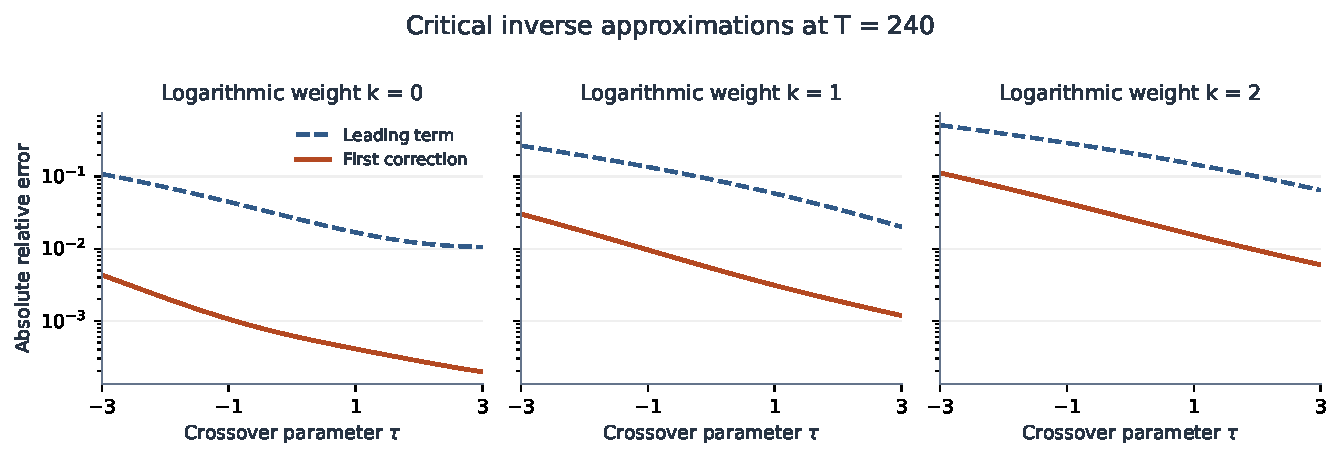
\includegraphics[width=\textwidth]{figures/critical_crossover_errors.pdf}
 \caption{Recorded errors for the weighted critical inverse at \(T=240\).
 Curves compare finite asymptotic truncations with numerical positive
 inverses at 183 sampled parameter choices.  They illustrate asymptotic
 accuracy and its dependence on the fixed logarithmic weight;
 they are not interval-certified bounds.}
 \label{fig:crossover}
 \end{figure}
}{}

\subsection{Rebuilding the package}

The article is built with ordinary pdfLaTeX; its bibliography is
embedded.  The supplied scripts use Python, mpmath, SymPy, and
Matplotlib, with versions listed in \path{verification/requirements.txt}.
The default verification output goes under \path{build/verification};
it does not overwrite the recorded data.
The README gives the exact commands.
The recorded checks are finite algebraic equalities or
high-precision diagnostics.  Neither floating-point residuals nor
agreement of two implementations substitutes for the quantified
proofs in this article.

\section{Further research questions}
\label{sec:questions}

\paragraph{1. Uniform coefficient extraction at the critical order.}
Theorem~\ref{thm:critical} is an inverse-germ theorem for
\(\eps T\) bounded.  Derive an analogue of
Theorem~\ref{thm:coeff-dilog} in a joint limit of the coefficient
index and the order, retaining the entire function \(H_k\).
The relevant coefficient scale need not be obtained by simply
replacing \(T\) with \(\log n\).

\paragraph{2. The nonlinear feedback endpoint with logarithmic weights.}
Insert the cancelled normal form into the repository's critical
feedback equations and prove the corresponding coefficient and
cutoff theorems.  The bare inverse established here is one analytic
ingredient; the conditioning and global coefficient analysis remain
separate tasks.

\paragraph{3. Growing logarithmic weights.}
Allow \(k=k(T)\) with \(k/T\) or \(k/\log T\) of order one.
The positivity of \(H_k\) persists on the real axis, but the
implicit-function neighborhoods used here are not uniform in \(k\).
The integral defining \(H_k\) suggests a second saddle analysis.

\paragraph{4. Large-order behavior of the reciprocal Gamma coefficients.}
Determine the growth, signs, and optimal truncation of
\[
 c_j=-[z^{j+1}]\Gamma(z-j-1)^{-1}.
\]
The differentiation order and the negative evaluation point grow
together.  A fixed-point Taylor estimate for \(1/\Gamma\) does not
settle this problem.  Determine whether a suitable summation or
acceleration reconstructs the coefficient expansion.

\paragraph{5. Complex zeros of the crossover profile.}
Near \(H_k(\tau_*)=0\), construct the replacement for
\eqref{eq:critical-chart}.  The leading normalized forward coefficient
vanishes and the normalization \(1/H_k\) diverges, so a new balance is
required.  Classify simple and multiple zeros and
the resulting local powers and logarithms.

\paragraph{6. Uniform higher-integer resonance with weights.}
Combine the exact pair \eqref{eq:respair} with the weighted inverse
lift while \(s\to m+1\), \(m\ge2\), and
\((s-m-1)\log(1/y)\) remains bounded.
The unweighted order-three feedback case has a repository predecessor;
the full weighted inverse coefficient transition remains to be worked out.

\paragraph{7. Noninteger logarithmic weights.}
For real or complex \(\kappa\), replace \((\log\nu)^k\) by
\((\log\nu)^\kappa\), with the first few terms treated separately.
Integer order differentiation is no longer a finite exact operation.
Determine when a finite holomorphic chart survives and when only an
asymptotic or integral representation is available.

\paragraph{8. Mixed polylogarithmic tails and cancellation of the boundary.}
For finite sums of dilated polylogarithms and order derivatives,
classify the cancellations that remove the highest logarithmic
polynomial.  Determine the replacement support law when \(b=0\) and
the first nonzero singular term occurs at a later power.

\paragraph{9. Global geometry beyond integer orders.}
Lemma~\ref{lem:univalence} holds for every real \(s>1\), but the
simple cut-modulus argument was used here for integers.
Prove a corresponding sharp endpoint-circle theorem for all real
orders, or identify the exact range where it fails.
This would extend the coefficient conclusions beyond the resonant cases.

\paragraph{10. Effective radii for the convergent charts.}
Compute explicit polydisc radii and outward-rounded bounds for the
implicit equations in Sections~\ref{sec:weighted} and
\ref{sec:critical}.  The existing Cauchy estimates prove existence
and error shape; they do not give ready-to-use certified numerical
constants.

\paragraph{11. Multiple polylogarithms.}
Investigate endpoint inverses of one-variable multiple polylogarithms
whose local expansions have several independent logarithmic blocks.
The general polynomial-logarithmic inverse theorem applies once an
exact normal form with a nonzero linear term is established, but
the depth dependence and possible cancellations require a separate analysis.

\paragraph{12. Formalization and symbolic certification.}
A realistic first Lean target is the finite support-counting argument
\eqref{eq:support-count} and the Fuss--Catalan corner extraction.
The analytic convergence, holomorphic implicit-function theorem, and
singularity transfer are larger formalization tasks.
A symbolic implementation should retain the exact resonant pair
until a parameter regime is specified, so it cannot silently replace
a uniform expression by a nonuniform finite jet.

\appendix
\section{Proof dependencies and mathematical status}

\begin{longtable}{@{}>{\raggedright\arraybackslash}p{.27\textwidth}
 >{\raggedright\arraybackslash}p{.38\textwidth}
 >{\raggedright\arraybackslash}p{.25\textwidth}@{}}
\toprule
Result & Essential input & Type of conclusion\\
\midrule
\endhead
Resonant order jets &
Classical Jonqui\`ere identity, Gamma recurrence, normal convergence &
Exact identity on a slit disc\\
Weighted inverse and corner law &
Holomorphic implicit function theorem, support counting, Lagrange inversion &
Convergent chart and exact coefficients\\
Uniform critical inverse &
Pole-cancelled weighted identity, nonvanishing \(H_k\), compact parameter set &
Convergent uniform chart for fixed \(k\)\\
First exponential block &
Analytic divisibility in the third chart variable &
Difference from the complete logarithmic block\\
Global coefficient domain &
Positive-imaginary integral, cut-modulus gap, growth at infinity &
Univalence, exact radius, dented continuation\\
Higher inverse coefficients &
Convergent local inverse, Gamma quotient, singularity transfer &
All fixed orders of an asymptotic expansion\\
Dilogarithm coefficients &
Fixed keyhole gap, local rescaling, integrable Taylor remainders &
All fixed orders in the Lambert scale\\
Computational files &
Exact finite algebra and arbitrary-precision evaluations &
Reproducibility and diagnostics\\
\bottomrule
\end{longtable}

The proposed new content lies in the explicit combinations and
conclusions described in Section~\ref{sec:intro}.  The table is also a
list of what would have to be formalized or independently checked to
upgrade the package to a machine-verified development.

\section{A useful finite-series recurrence}

For numerical reproduction of individual inverse coefficients, let
\[
 f(z)=\frac{\Li_s(z)}z=\sum_{j\ge0}f_jz^j,\qquad
 f_j=(j+1)^{-s},\qquad
 f(z)^{-n}=\sum_{j\ge0}h_jz^j.
\]
Then \(h_0=1\), and differentiation of \(f h'=-n f'h\) gives
\begin{equation}
 h_k=\frac1k\sum_{j=1}^k\bigl((1-n)j-k\bigr)f_jh_{k-j},
 \qquad a_n^{(s)}=\frac{h_{n-1}}n.
 \label{eq:finite-recurrence}
\end{equation}
For integer \(s\), the recurrence can be evaluated exactly over
\(\mathbb Q\).  For high-precision floating arithmetic, cancellation
can be severe; agreement at two working precisions is a diagnostic
against that loss, not a rigorous rounding bound.

\begingroup
\small
\begin{thebibliography}{20}

\bibitem{dlmf-poly}
F. W. J. Olver et al., eds.,
\emph{NIST Digital Library of Mathematical Functions},
Section 25.12, especially equations 25.12.11--25.12.13.
\url{https://dlmf.nist.gov/25.12}.
Accessed 12 October 2026.

\bibitem{dlmf-w}
F. W. J. Olver et al., eds.,
\emph{NIST Digital Library of Mathematical Functions},
Section 4.13, Lambert \(W\)-function.
\url{https://dlmf.nist.gov/4.13}.
Accessed 12 October 2026.

\bibitem{dlmf-gamma}
F. W. J. Olver et al., eds.,
\emph{NIST Digital Library of Mathematical Functions},
Sections 5.5 and 5.11, Gamma reflection and asymptotic expansions.
\url{https://dlmf.nist.gov/5.5},
\url{https://dlmf.nist.gov/5.11}.

\bibitem{kr}
C. Krattenthaler and T. Rivoal,
\emph{On the compositional inverse of polylogarithms},
unpublished author-hosted note, dated 10 February 2025, 6 pp.
\url{https://rivoal.perso.math.cnrs.fr/articles/inversepolylog.pdf}.
Inspected version and normalization corrections are specified in
Section~\ref{sec:audit}.

\bibitem{fs}
P. Flajolet and R. Sedgewick,
\emph{Analytic Combinatorics},
Cambridge University Press, 2009.
Chapters VI and VIII, and Appendix A.
Author-hosted text:
\url{https://algo.inria.fr/flajolet/Publications/book.pdf}.

\bibitem{repo-poly}
V. Reshetnikov, ProveIt research collection,
\emph{Analysis/Polylogarithms}.
Inspected manuscript chapters include
\path{01-foundations.tex},
\path{07-tornheim-evaluation.tex},
\path{07-shifted-stieltjes-correlations.tex},
\path{08-periodic-collision-contacts.tex}, and
\path{11-literature.tex}.
\url{https://github.com/VladimirReshetnikov/ProveIt/tree/9ec0f0406afe7a5475b03ff65ed91f7e283979b8/Analysis/Polylogarithms}.

\bibitem{repo-lambert}
ProveIt research collection,
\emph{Logarithmic Critical Endpoint Lambert Charts},
especially its general logarithmic inverse theorem.
\url{https://github.com/VladimirReshetnikov/ProveIt/tree/9ec0f0406afe7a5475b03ff65ed91f7e283979b8/Analysis/Transseries/docs/series-and-transseries/Logarithmic_Critical_Endpoint_Lambert_Charts}.

\bibitem{repo-confluent}
ProveIt research collection,
\emph{Confluent Critical Transseries Across the Exponent-Two Boundary},
especially the pole-cancelled normal form and holomorphic inverse chart.
\url{https://github.com/VladimirReshetnikov/ProveIt/tree/9ec0f0406afe7a5475b03ff65ed91f7e283979b8/Analysis/Transseries/docs/series-and-transseries/Confluent_Critical_Transseries_Exponent_Two_Boundary}.

\bibitem{repo-transport}
ProveIt research collection,
\emph{Nonlinear Stokes Transport and Logarithmic Inversion},
especially its analytic inverse-transport theorem.
\url{https://github.com/VladimirReshetnikov/ProveIt/tree/9ec0f0406afe7a5475b03ff65ed91f7e283979b8/Analysis/Transseries/docs/series-and-transseries/Nonlinear_Stokes_Transport_Logarithmic_Inversion}.

\bibitem{repo-slow}
ProveIt research collection,
\emph{Slowly Varying Action Tails and Critical Transseries},
Section 8 and Research Question 5.
\url{https://github.com/VladimirReshetnikov/ProveIt/tree/9ec0f0406afe7a5475b03ff65ed91f7e283979b8/Analysis/Transseries/docs/series-and-transseries/Slowly_Varying_Action_Tails_Critical_Transseries}.

\end{thebibliography}
\endgroup
\end{document}
